%%%%%%%%%%%%%%%%%%%%%%%%%%%%%%%%%%%%%%%%%%%%%%%%%%%%%%%%%%%%%%%%%%%%%%%%%
\subsection{Motivation: spatial locality in KV-storage} 
%%%%%%%%%%%%%%%%%%%%%%%%%%%%%%%%%%%%%%%%%%%%%%%%%%%%%%%%%%%%%%%%%%%%%%%%%

% KV-stores are everywhere
Key-value stores (KV-stores) are widely used  by a broad range of applications and are projected
to continue to increase in popularity in years to come; market research  identifies them as the 
``driving factors'' of the NoSQL market, which is expected to garner \$4.2B by 2020~\cite{alliedmarketresearch}.

% In many applications, keys are composite
KV-stores provide a simple programming model. 
Data is an ordered collection of key-values pairs, and  the API supports random writes, 
random reads, and range queries. 

A common design pattern is the use of \emph{composite} keys that represent an agglomerate of attributes.
Typically, the first attribute -- called the \emph{primary key} -- has a skewed distribution, and so   access via the composite key exhibits \emph{spatial locality}, as 
popular primary keys result in popular \emph{key ranges}. 

One example of this arises in real-time mobile analytics platforms such as Google Analytics or Flurry Analytics.   
These platforms ingest massive streams of event reports (e.g., app start/stop,  exercising a particular code path within an app) from over a billion mobile users.  
% starting or stopping an app, exercising a particular code path within an app,  clicking on an ad, etc. 
The data store is indexed by a composite key consisting of  app name (or id) and additional attributes (user id, device, time, location, event type, etc.) 
%The query API is app id-centric, hence this dimension is the key prefix.
We examine a real trace of  $200$ million events captured from a production mobile analytics engine over the course of $4$ minutes.  
\Cref{fig:cdf} shows the distribution of app names in this stream.  
Although the stream includes reports from $40$K apps, 
we find that $10$\% of the apps cover over $99.5$\% of the events; $1$\% of the applications cover $94$\% of the events; and less than $0.1$\% cover $70$\% of the events. 
% This means the data is highly skewed and with a very long tail (not depicted in the figure).
%Table~\ref {table:popular} shows the cumulative probability of the top-$20$ popular applications, covering more than $50$\% of the events. 
%With application name as the primary dimension of a composite key this distribution induces high spatial locality.


\begin{figure}[tb]
\centering
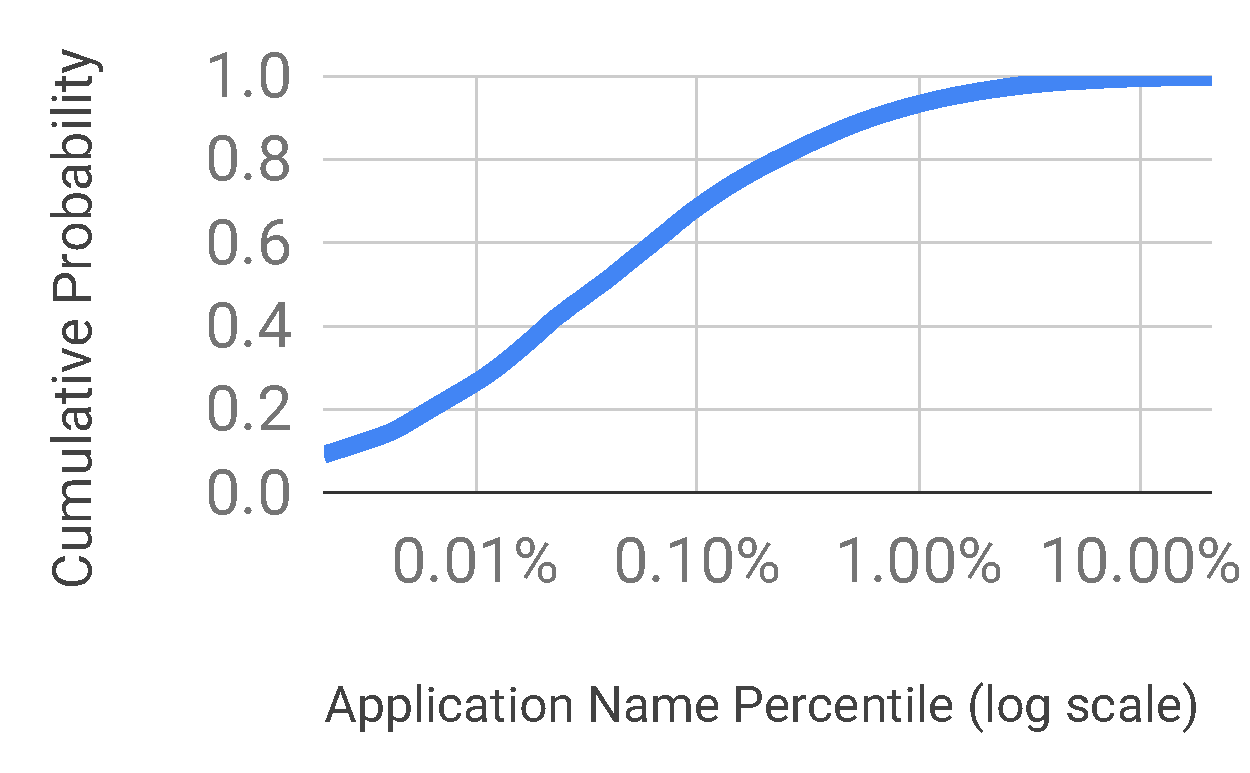
\includegraphics[width=0.75\columnwidth]{figs/cdf.pdf}
\caption{CDF of app names in a real-world mobile analytics event stream consisting of 200 million events.}
\label{fig:cdf}
\end{figure}

Composite keys arise in many additional domains, including messaging and social networks. 
For example a query in Facebook Messenger may retrieve the last 100 messages for a 
given user~\cite{Borthakur:2011:AHG:1989323.1989438}, where the primary key is user id. 
In Facebook's social network, a graph edge is indexed by a key consisting of two 
object ids and an association type~\cite{Armstrong:2013:LDB:2463676.2465296}.
Note further that spatial locality  arise also with simple (non-composite) keys, for example, when 
reverse  URL domains are used as keys for web  indexing~\cite{Cho:1998:ECT:297805.297835}. 

% Overfitting for Zipf 
The prevalence of skewed  access  in real workloads is widely-recognized, 
and indeed standard benchmarks (e.g., YCSB~\cite{YCSB})  feature skewed key-access distributions like Zipf.
But 
these benchmarks fail to capture the spatial aspect of locality.
This, in turn, leads to storage systems being optimized for a skewed distribution on individual keys with no spatial locality,
e.g., by partitioning data by recent access time as opposed to by key.
In this work, we make spatial locality a first class consideration in KV-store design.
% which leads us to rethink the design principles underlying today's popular KV-stores.

% LSM is the standard but not ideal for this  because of  write path  temporal grouping leading to fragmentation and write amplification
The de facto standard approach to building KV-stores today is \emph{LSM} (log-structured merge) trees~\cite{DBLP:journals/acta/ONeilCGO96}. 
%The LSM approach optimizes write performance by absorbing random writes in memory and periodically flushing 
%them as sequential files to disk. %While  sequential disk access dramatically improves I/O throughput, it 
% is important to n
The LSM design initially groups writes  into files \emph{temporally}, and not by key-range. 
A background \emph{compaction} process later merge-sorts any number of files, grouping data by keys. 
This approach is not ideal for workloads with high spatial locality for two reasons. 
First,  popular key ranges are fragmented across many files. % during long periods (between compactions). 
Second,  compaction  is costly in terms of  both performance 
(disk bandwidth) and \emph{write amplification}, namely the number of physical writes 
associated with a single application write. The latter is  particularly important in SSDs as it increases disk wear. 
The temporal grouping means that compaction is indiscriminate with respect to key popularity:  
Since new (lower level) files are always merged with old (higher level) ones, 
 ``cold'' key ranges
 % that has not been accessed since the  beginning of time 
 continue to be repeatedly re-located
by  compactions.  

% LSM is not the best when the entire working set fits in memory
Additionally, we note that LSM's temporal  organization optimizes disk I/O but induces a penalty on in-memory operation. 
All keys -- including popular ones -- are flushed to disk periodically, even though persistence is assured 
via a separate \emph{write-ahead-log (WAL)}.
Beyond increasing write amplification, this makes the flushed keys unavailable for fast read from memory,
which is  wasteful if the system incorporates sufficient DRAM to hold most of the active working set. 
The drop in DRAM prices (more than $6.6$x since 2010~\cite{dram-prices})  
%and significant performance benefit DRAM offers 
makes the latter scenario increasingly common.  

%%%%%%%%%%%%%%%%%%%%%%%%%%%%%%%%%%%%%%%%%%%%%%%%%%%%%%%%%%%%%%%%%%%%%%%%%
\subsection{Designing for spatial locality} 
%%%%%%%%%%%%%%%%%%%%%%%%%%%%%%%%%%%%%%%%%%%%%%%%%%%%%%%%%%%%%%%%%%%%%%%%%

The main goal of this work is to draw attention to the importance of spatial locality in 
today's KV-store workloads and to propose a design alternative  that is better suited for such locality. 
Obviously, we do not claim that spatial data partitioning is new; indeed, classical B-trees~\cite{DBLP:conf/sigmod/BayerM70,Comer79} 
 pre-date  LSM trees, and many B-tree variants~\cite{Brodal:2003:LBE:644108.644201,Bender15, Lehman:1981:ELC:319628.319663} have  emerged over the years. 
 However, it is important to note that these trees are  conceptual constructs rather than storage systems; 
 employing these concepts within a practical data store over a memory hierarchy 
 raises multiple challenges,  which perhaps explains their limited adoption in industrial KV-stores.
 
A key challenge is what to persist when and in what format. 
In classical B-trees, all updates induce random I/O to leaves, resulting in poor write performance. 
A $B^{\epsilon}$-tree~\cite{Brodal:2003:LBE:644108.644201}  reduces this overhead using  write buffers in internal tree nodes. 
However, this slows down lookups, which now have to search in multiple unordered buffers. 
If internal  nodes reside on disk, the lookup time is unacceptably slow, whereas
if they reside in RAM then they have to be complemented by a separate persistence mechanism. 

A second challenge is ensuring consistency -- in particular, atomic scans --  in the face of concurrent access. 
This can be  tricky when a scan spans both memory-resident and disk-resident data.
In fact, we are not aware of any published solution addressing atomic scans and persistence with concurrent access (multi-threading) in  B- or  B$^\epsilon$-trees.

% Drum roll 
We present \sys, a high-performance persistent KV-store geared towards spatial locality. % whose design diverges from the ubiquitous LSM approach.  
We forgo LSM's temporal  organization and instead partition data by key, as in B- and B$^\epsilon$-trees. 
Data is organized  as a list (rather than a tree) of large \emph{chunks} holding contiguous key ranges.
An auxiliary volatile index provides direct access (one I/O operation) to the on-disk chunk holding a given key.  
\sys\ supports atomic scans using low-overhead multi-versioning, where versions are increased only by scans and not by updates. 

Like  LSMs,  \sys\ optimizes I/O by absorbing updates in memory before writing to disk. 
We achieve this without a temporal data organization thanks to (1) caching popular chunks in RAM and (2) using
per-chunk WALs to transform  random I/O to sequential I/O at the chunk level. 


% Benefits
Spatially-organized chunks have a number of advantages:
(1) there is little fragmentation of key ranges and hence better  performance for workloads with spatial locality; 
(2) in-memory chunk compaction saves  disk flushes and reduces write volume;  
(3) keeping hot ranges in memory leads to better performance, especially when most of the working set fits in RAM; and
(4) in-chunk WALs  allow quick recovery from crashes with no need to replay any WALs.

% Downsides
The downside of spatial partitioning is that if the data lacks spatial locality and the active working set is big, 
caching an entire chunk for a single popular key is wasteful. We mitigate this  by adding 
a dedicated \emph{row cache} for hot keys. But since the row cache only serves the read-path, 
this design is less optimal for mixed read/write workloads lacking spatial locality,
where the LSM approach may be more suitable.  

%%%%%%%%%%%%%%%%%%%%%%%%%%%%%%%%%%%%%%%%%%%%%%%%%%%%%%%%%%%%%%%%%%%%%%%%%
\subsection{Contributions and roadmap}
%%%%%%%%%%%%%%%%%%%%%%%%%%%%%%%%%%%%%%%%%%%%%%%%%%%%%%%%%%%%%%%%%%%%%%%%%

\sys\ is a novel KV-store, which organizes data differently from classical LSM, B-, and $B^{\epsilon}$-trees; \cref{sec:principles} presents our key design goals and choices. 
The \sys\ algorithm, detailed in \cref{sec:design}, supports concurrency among any number of threads performing put, get, and scan operations, as well as background maintenance (compaction). It ensures consistency and correct recovery from failures. 
We  provide details on its C++ implementation in \cref{sec:impl}. 

In~\cref{sec:eval}, we extensively evaluate \sys. 
We experiment with three types of workloads: (1) a production trace collected from a large-scale mobile analytics platform; 
(2)  workloads with synthetically-generated composite keys exercising the standard scenarios of the popular YCSB benchmark suite~\cite{YCSB};
and (3)  YCSB's traditional benchmarks, which employ simple (non-composite) keys.  
In all cases, we compare \sys\ to the recent (Oct 2018) release of RocksDB~\cite{RocksDB}, a mature industry-leading LSM KV-store. 
We further experimented with two additional open-source KV-stores, (1) the LSM-based PebblesDB~\cite{PebblesDB}, and (2) PreconaFT/TokuDB~\cite{TokuDB} -- the only
publicly-available KV store that uses a $B^{\epsilon}$-tree design. However, both of these performed significantly worse than both RocksDB and \sys\ across 
the entire YCSB benchmark suite, which is in line with previous studies of PerconaFT~\cite{tucana}, so we excluded them from further tests. 

Our experiments show the following: (1) \sys\/ significantly outperforms RocksDB when spatial  locality is high.  
For instance, on a 256GB production dataset, \sys\ ingests data 3.7x faster than RocksDB,  scans recent  data up to 27\% faster, 
and reduces write amplification by nearly 4x. 
And in large synthetic composite-key workloads, \sys\  improves over RocksDB's throughput by $24\% - 75\%$. 
(2) \sys\/ significantly outperforms RocksDB whenever most of the working set fits in RAM. 
For example, with synthetic composite keys and a memory-resident 
working set, \sys\  accelerates scans by up to $3.5$x, puts by up to $2.3$x, and gets by up to $2$x. 
(3) In traditional YCSB workloads,  \sys\ is comparable to RocksDB. As can be expected, RocksDB performs better than 
\sys\ in mixed read/write workloads with large active working sets and no spatial locality. 


Finally,~\cref{sec:related}  surveys related work and~\cref{sec:conclusions} concludes. 
